\documentclass[a4paper,fleqn]{cas-sc}

\usepackage[authoryear]{natbib}
\usepackage{amsmath,amssymb}
\usepackage{booktabs}
\usepackage{threeparttable}
\usepackage{graphicx}
\usepackage{multirow}
\usepackage{lineno}
\usepackage[section]{placeins}
\usepackage{xcolor}
\usepackage{setspace}
\usepackage{float}

\ExplSyntaxOn
\cs_new_eq:NN \lr_cusum_original_make_tbl_caption:nn \__make_tbl_caption:nn
\cs_set:Npn \__make_tbl_caption:nn #1#2
  {
    \group_begin:
      \skip_set:Nn \l_tbl_abovecap_skip {3pt}
      \setstretch{1.5}
      \lr_cusum_original_make_tbl_caption:nn {#1} {#2}
    \group_end:
  }
\cs_new_eq:NN \lr_cusum_original_make_fig_caption:nn \__make_fig_caption:nn
\cs_set:Npn \__make_fig_caption:nn #1#2
  {
    \group_begin:
      \skip_set:Nn \l_fig_abovecap_skip {3pt}
      \setstretch{1.5}
      \lr_cusum_original_make_fig_caption:nn {#1} {#2}
    \group_end:
  }
\ExplSyntaxOff

\begin{document}
\linenumbers

\let\WriteBookmarks\relax
\def\floatpagepagefraction{1}
\def\textpagefraction{.001}

\shorttitle{Windowed CUSUM analysis of near-decadal Sentinel-1 SAR time series}
\shortauthors{Rao et al.}

% TODO(author): Confirm corresponding-author marks and email assignments before submission.
\author[1]{Keyi Rao}[orcid=0000-0001-8443-9819]\cormark[1]
\credit{Conceptualization, Methodology, Software, Data curation, Formal analysis, Project administration, Writing -- original draft, Visualization}

\author[1]{Shixin Dong}[orcid=0009-0005-7299-5312]\cormark[1]
\credit{Software, Visualization, Validation, Writing -- review and editing}

\author[2]{Zhongwen Hu}[orcid=0000-0003-2689-3196]
\credit{Supervision, Validation, Funding acquisition}

\author[3,4]{Cesar Ivan Alvarez}[orcid=0000-0001-5629-0893]
\credit{Conceptualization, Methodology, Writing -- review and editing}

\author[1]{Zhaocong Wu}[orcid=0000-0003-2435-5538]
\ead{zcwoo@whu.edu.cn}
\credit{Conceptualization, Supervision, Funding acquisition}

\affiliation[1]{organization={School of Remote Sensing and Information Engineering, Wuhan University},
  addressline={No. 299 Bayi Road, Wuchang District}, city={Wuhan}, postcode={430072},
  state={Hubei}, country={China}}
\affiliation[2]{organization={School of Architecture and Urban Planning and MNR Key Laboratory for Geo-Environmental Monitoring of Great Bay Area, Shenzhen University},
  addressline={No. 3688 Nanhai Avenue, Nanshan District}, city={Shenzhen},
  postcode={518060}, state={Guangdong}, country={China}}
\affiliation[3]{organization={Institute of Geography, Faculty of Applied Informatics, University of Augsburg},
  addressline={Universit\"atsstra\ss e 12}, city={Augsburg}, postcode={86159}, country={Germany}}
\affiliation[4]{organization={Maestr\'ia en Sistemas de Informaci\'on Geogr\'afica, Topograf\'ia Automatizada y Fotogrametr\'ia Digital, Universidad Cat\'olica de Santiago de Guayaquil},
  city={Guayaquil}, country={Ecuador}}
\cortext[cor1]{Corresponding author}

\title[mode=title]{Windowed CUSUM analysis of near-decadal Sentinel-1 SAR time series for monitoring recurrent stand disturbances in Ecuadorian balsa plantations}

% \begin{abstract}
% Short-rotation balsa \textit{Ochroma pyramidale} plantations require temporally explicit disturbance histories rather than a single forest-loss label, yet persistent cloud cover limits optical continuity in tropical regions. We developed Windowed CUSUM, a local-reference framework that combines overlapping temporal windows, central-interval admission, directional screening, permutation-based statistical support, and event consolidation to reconstruct recurrent stand disturbances from near-decadal Sentinel-1 time series. The framework was evaluated against 1,093 month-resolved reference events from 462 plantation polygons grouped into 57 spatial blocks and then applied to 3,498 validated polygons across Ecuador. Historical disturbances showed consistent within-stand declines despite substantial overlap in absolute backscatter, with median post-minus-pre-event changes of about $-1.5$ dB in both VV and VH. Under nested five-fold spatial out-of-fold evaluation, Windowed CUSUM achieved a precision of 0.789, recall of 0.806, F1 of 0.797, and temporal mean absolute error of 0.776 months. The strongest benchmark, decrease-filtered ReCuSum, achieved an F1 of 0.675; the gain arose mainly from higher recall. Component analyses identified local-reference windowing as the main source of recurrent-event sensitivity, while central-interval admission and permutation screening mainly improved precision. Temporal truncation showed recall of 0.790 after six post-disturbance months, with 96.8\% of those detections remaining within two months of their 12-month dates. Across the validated inventory, the locked VV-only detector identified 6,658 disturbances during 2017--2025 and 3,509 consecutive inter-disturbance intervals, with a median recurrence of 36 months. Proposed Windowed CUSUM therefore extends near-decadal SAR monitoring from individual disturbance detection toward reconstruction of recurrent plantation disturbance histories.
% \end{abstract}

% Balsa plantations have rapid management turnover, but persistent tropical cloud cover limits optical reconstruction of repeated stand disturbances. 
\begin{abstract}
  Short-rotation balsa \textit{Ochroma pyramidale} plantations require temporally explicit disturbance histories rather than a single forest-loss label, yet persistent cloud cover limits optical continuity in tropical regions. We developed Windowed CUSUM, a locally adaptive cumulative-sum framework that combines geometry-consistent, track-specific Sentinel-1 trajectories with temporal and statistical adaptation. Overlapping windows repeatedly renew the local temporal reference, while a window-specific permutation null calibrates each observed CUSUM amplitude against the variability of the same local context. Centrally admitted, statistically supported candidates are then consolidated across overlapping windows and tracks into recurrent stand-disturbance histories. Evaluation used 1,093 reference events with month-level timing from 462 polygons grouped into 57 spatial blocks. Historical disturbances showed repeatable within-stand backscatter declines despite substantial overlap in absolute VV and VH states. Under five-fold spatial out-of-fold evaluation, Windowed CUSUM achieved precision 0.789, recall 0.806, F1 0.797, and matched-event MAE 0.776 months, compared with F1 0.680 for CCDC VV and 0.675 for decrease-filtered ReCuSum. The paired F1 advantage over ReCuSum was $+0.122$ (95\% CI: 0.094--0.149), driven mainly by higher recurrent-event recall. Component analysis identified local-reference renewal as the main source of sensitivity, while central event admission and local statistical calibration recovered precision. With six months of post-event observations, recall reached 0.790, and 96.8\% of events already detected by that horizon were dated within two months of their 12-month estimates. Applied to 3,498 validated balsa polygons, the framework reconstructed 6,658 disturbances and 3,509 consecutive inter-disturbance intervals during 2017--2025, with a median recurrence of 36 months. The framework extends cloud-independent SAR monitoring from isolated disturbance detection toward reconstruction of recurrent plantation disturbance histories.
\end{abstract}

\begin{highlights}
\item Recurrent balsa disturbances show consistent within-stand Sentinel-1 declines
\item Windowed CUSUM reconstructs recurrent disturbances from near-decadal SAR records
\item Local-reference windowing is the main source of recurrent-event sensitivity
\item Windowed CUSUM reaches 0.806 recall versus 0.591 for the strongest benchmark
\item Median observed inter-disturbance recurrence is 36 months
\end{highlights}

\begin{keywords}
Balsa plantation \sep Sentinel-1 \sep CUSUM \sep forest disturbance \sep spatial validation \sep short-rotation forestry
\end{keywords}

\maketitle
\doublespacing


% !TeX root = ../main.tex
\section{Introduction}
\label{sec:introduction}

Balsa (\textit{Ochroma pyramidale}) is a fast-growing tropical tree species whose lightweight wood is widely used as a core material in applications such as wind turbine blades~\citep{Midgley2010Balsa,Jenkin2019BalsaValueChain,Borrega2015Balsa_mechanics}. Ecuador is a major source of commercial balsa, where plantation stands can undergo management-related turnover on cycles of only a few years under productive tropical conditions~\citep{GonzalezOsorio2010Balsa,CanadasLopez2019BalsaGrowth}. Reconstructing these short-rotation dynamics therefore requires a long and temporally continuous observation record capable of resolving multiple disturbance events within the same stand, rather than a single forest-loss label~\citep{CanadasLopez2019BalsaGrowth,Jenkin2019BalsaValueChain}. This requirement is difficult to meet with optical imagery because persistent cloud cover in tropical Ecuador disrupts temporal continuity and can leave critical disturbance periods unobserved. Together, rapid plantation turnover and persistent cloud cover make long-term, cloud-independent SAR observations essential for reconstructing plantation rotation dynamics~\citep{Reiche2018Bayesian,Doblas2020harmonic,Matthew2021BFAST,Bullock2022CCDC_S1,FLORES2026Sensitivity}. The near-decadal Sentinel-1 archive provides the temporal continuity~\citep{Torres2012S1} needed to investigate whether recurrent stand disturbances can be reliably resolved from long-term SAR trajectories.

Long-term plantation management histories have been reconstructed primarily from optical satellite archives. Multi-decadal Landsat records have been used to identify the starts and ends of successive rotations and quantify productivity across thousands of \textit{Eucalyptus} stands~\citep{McMahon2019EucalyptusRotations}, while other time-series approaches have retrieved planting history, harvest timing, generation, rotation length, and stand age in short-rotation plantations~\citep{Du2022GlobalPlantingYears,Li2022EucalyptusHistory}. More recent studies have moved toward denser temporal characterization, including biweekly monitoring of industrial plantation dynamics from PROBA-V~\citep{Bos2025PlantationDynamics} and month-resolved harvest dating and stand-age estimation from Harmonized Landsat--Sentinel imagery~\citep{Huang2026EucalyptusAge}. Sentinel-1 research has developed largely along a complementary trajectory, emphasizing forest disturbance detection and near-real-time warning under cloudy conditions. Dense Sentinel-1 time series have supported probabilistic deforestation monitoring~\citep{Reiche2018Bayesian}, continuous CUSUM-based detection~\citep{RuizRamos2020CUSUMSMC,Ygorra2021CuSum}, selective-logging and plantation-harvest detection~\citep{Matthew2021BFAST,Xulu2020PlantationHarvest}, operational alert systems~\citep{Doblas2022DETERR,Bullock2022CCDC_S1,Mullissa2024LUCA}, and recursive identification of multiple tropical forest disturbances~\citep{Ygorra2023ReCuSum}. Despite these advances, the use of a near-decadal Sentinel-1 record to reconstruct multiple disturbance events within the same managed stand, and thereby recover rotation-relevant histories for a short-rotation plantation system, remains largely unexplored.

Even with dense SAR observations, reconstructing recurrent disturbance events remains challenging. Sentinel-1 backscatter responds not only to canopy structure but also to rainfall and moisture, surface roughness, acquisition geometry, and phenological state, producing temporal variability that can overlap the signal of structural change ~\citep{Doblas2020harmonic,Reiche2018Bayesian,Matthew2021BFAST,vanDerWoude2024S1Disturbance,FLORES2026Sensitivity}. Similar absolute backscatter values may therefore occur under different plantation states, limiting the transferability of a single threshold of backscattering coefficient across stands and environments. After disturbance and subsequent recovery, a fixed historical reference may also cease to represent the current stand condition. CUSUM is feasible because it accumulates persistent departures from an explicit reference state~\citep{Page1954CUSUM}, and Sentinel-1 applications have demonstrated its utility for sustained forest-cover change~\citep{RuizRamos2020CUSUMSMC,Ygorra2021CuSum}. ReCuSum extends this principle to multiple changes through recursive segmentation~\citep{Ygorra2023ReCuSum}, although later segments depend on previously estimated boundaries and may contain progressively fewer observations. For short-rotation plantations, the central methodological challenge is therefore to detect successive disturbances relative to each stand's recent temporal background while maintaining accurate month-level event timing.

These challenges motivate a recurrent-event framework that repeatedly updates each stand's local temporal background as the time series evolves, allowing successive disturbances to be detected relative to the stand's current condition rather than a fixed historical baseline. We therefore propose \textit{Windowed CUSUM}, which implements this principle through overlapping local-reference windows and retains only centrally located negative departures with statistical support before consolidating them into a recurrent disturbance history. This study aims to (1) characterize the within-stand Sentinel-1 response to historical balsa disturbances; (2) evaluate whether Windowed CUSUM improves recurrent-event detection relative to alternative detectors and remains robust to stand representation, polarization, temporal configuration, and statistical assumptions; and (3) reconstruct recurrent plantation disturbance histories and characterize their spatial and temporal dynamics using stand-level event counts and inter-disturbance intervals (Fig.~\ref{fig:national_recurrence_patterns}).
\begin{nolinenumbers}
\begin{figure}[pos=!htbp]
    \centering
    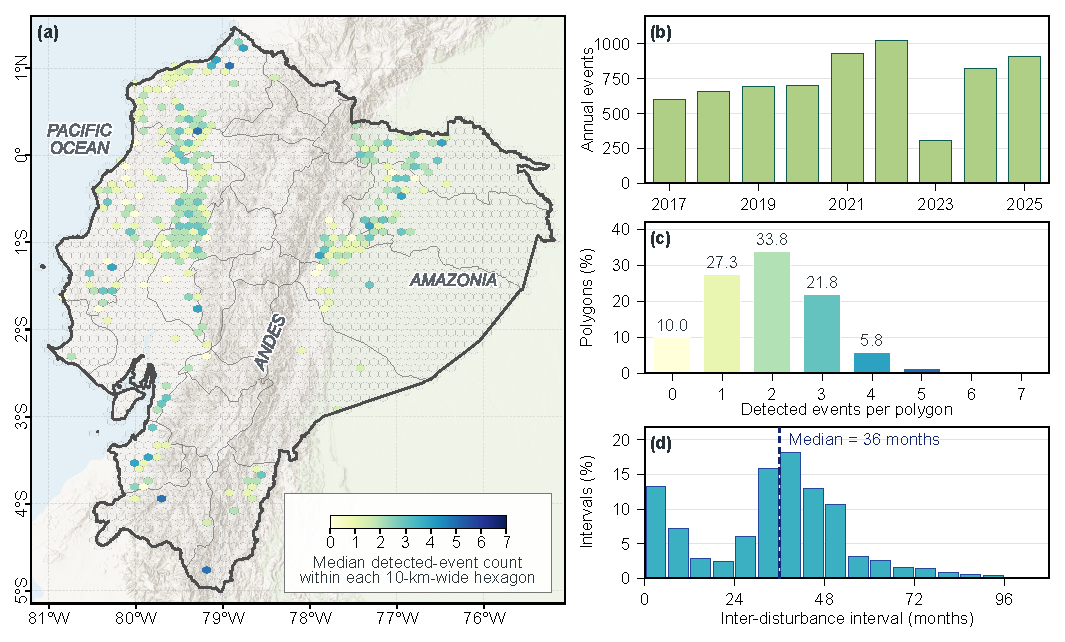
\includegraphics[width=0.92\linewidth]{figures/fig01_national_recurrence.pdf}
    \caption{Recurrent stand-disturbance patterns reconstructed by Windowed CUSUM across the Ecuadorian balsa plantations. (a) Spatial pattern of stand-disturbance recurrence. (b) National annual stand-disturbance frequency. (c) Number of detected disturbances per balsa plantation. (d) Intervals between consecutive detected stand-disturbances; the dashed line indicates the median.}
    \label{fig:national_recurrence_patterns}
\end{figure}
\end{nolinenumbers}




\FloatBarrier

% !TeX root = ../main.tex
\section{Study area and data}
\label{sec:materials}

\subsection{Study area and BALSA plantation inventory}
\label{sec:study_area_inventory}

The study covered mainland Ecuador, with particular emphasis on the humid Pacific lowlands and western Andean foothills where commercial BALSA plantations are concentrated as shown in Fig.~\ref{fig:study_area}. Balsa plantation boundaries were obtained from the Ecuadorian Ministry of Agriculture and Livestock through the Geoportal del Agro Ecuatoriano (\url{https://geoportal.agricultura.gob.ec/}).

\begin{figure}[pos=!htbp]
    \centering
    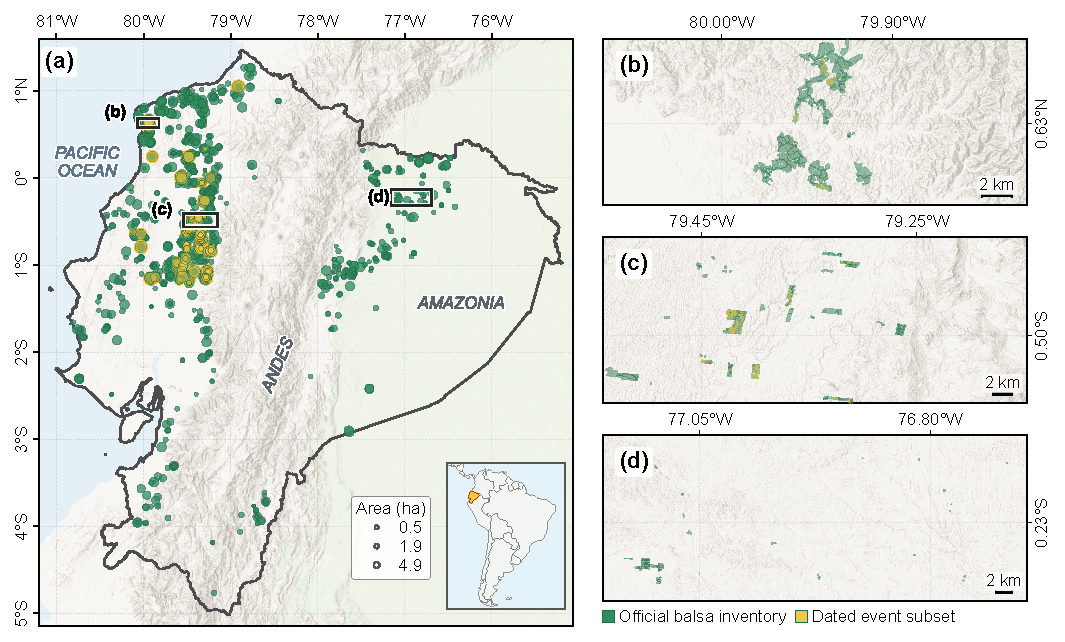
\includegraphics[width=0.92\linewidth]{figures/fig02_study_area.pdf}
    \caption{Study region and official BALSA plantation inventory. Green markers show all 3,890 BALSA polygons, and yellow markers identify the subset containing dated stand-disturbance events. Panels (b)--(d) enlarge representative plantation regions.}
    \label{fig:study_area}
\end{figure}

The source forestry inventory contained 26,206 plantation polygons, of which 3,498 carried the species label BALSA and marked VALIDADO. The validated balsa inventory covered 13,651.85~ha and was divided into three fixed size classes for stratified reporting: small ($\leq1$~ha), medium ($>1$--5~ha), and large ($>5$~ha) (Table~\ref{tab:inventory}).

\begin{table}[pos=!htbp]
    \centering
    \caption{Polygon counts and mapped area by size class for the 3,498 validated BALSA plots in UTM zone 17S (EPSG:32717).}
    \label{tab:inventory}
    \begin{threeparttable}
    \begin{tabular}{lrrrrr}
        \toprule
        Class & Polygons & Polygons (\%) & Area (ha) & Area (\%) & Median (ha) \\
        \midrule
        Small ($\leq1$ ha) & 1,325 & 37.88 & 497.38 & 3.64 & 0.30 \\
        Medium ($>1$--5 ha) & 1,385 & 39.59 & 3,556.10 & 26.05 & 2.33 \\
        Large ($>5$ ha) & 788 & 22.53 & 9,598.37 & 70.31 & 8.68 \\
        \midrule
        Total & 3,498 & 100.00 & 13,651.85 & 100.00 & -- \\
        \bottomrule
    \end{tabular}
    \end{threeparttable}
\end{table}


\subsection{Sentinel-1 OPERA RTC-S1 archive and analytical coverage}
\label{sec:s1_archive}

Sentinel-1 observations were obtained from the NASA OPERA Level-2 Radiometric Terrain Corrected Sentinel-1 (RTC-S1) archive~\citep{shiroma2023OPERARTC,opera2023rtc} and organized using S1-GRiTS v3.0.0 (\url{https://github.com/ottoKae/S1-GRiTS}). OPERA RTC-S1 provides burst-based, radiometrically terrain-corrected $\gamma^{0}$ backscatter at 30-m pixel spacing for VV and VH polarizations.

The Sentinel-1SAR archive in Ecuador contained four relative Sentinel-1 tracks in ascending orbit (TK18, TK47, TK91, and TK120). Native observations began between May and October 2016, depending on the tile--track combination. Observations were indexed on a common monthly calendar from January 2016 to June 2026 while preserving each track's native temporal support; months before a track's first observation or after its final observation remained missing. The historical evaluation interval was fixed to January 2017--December 2025, while observations outside this interval provided temporal context for the windowed detector and the subsequent prospective replay.

The 3,498 validated BALSA polygons intersected 40 tile--track combinations, yielding 4,001 polygon--track objects for time-series extraction. Track identity was preserved throughout time-series construction and disturbance detection so that observations from different relative orbits or viewing geometries were not mixed before event consolidation. Detailed acquisition-level compositing, missing-data handling, and stand-level aggregation are described in Section~\ref{sec:s1_timeseries_representation}.


\subsection{Historical disturbance dated-reference}
\label{sec:historical_references}

Historical disturbance months were assigned by visual interpretation and reconciled to the frozen polygon identifiers. Single-date PlanetScope imagery (approximately 3~m) was the primary evidence source, with monthly Planet basemaps (approximately 4.77~m at the Equator) used where appropriate (Fig~\ref{fig:s1_population_signatures}). Orbit-specific Sentinel-1 observations provided supplementary evidence when cloud cover or incomplete optical observations prevented an unambiguous optical-only date assignment. Interpretation was performed without access to Windowed CUSUM predictions, and ambiguous disturbance dates were not forced into the reference catalogue. After exact polygon--month duplicates were reconciled, the historical catalogue contained 1,093 reference-dated events in 462 validated BALSA polygons distributed across 57 spatial blocks within the 2017--2025 historical evaluation period.


% !TeX root = ../main.tex
\section{Methods}\label{sec:methods}



We developed Windowed CUSUM to detect recurrent stand disturbances from near-decadal Sentinel-1 time series and reconstruct plantation turnover histories. The workflow comprised stand-level time-series construction, recurrent-event detection, spatially structured evaluation, and rotation-history reconstruction (Fig.~\ref{fig:workflow}).


\begin{figure}[pos=!htbp]
    \centering
    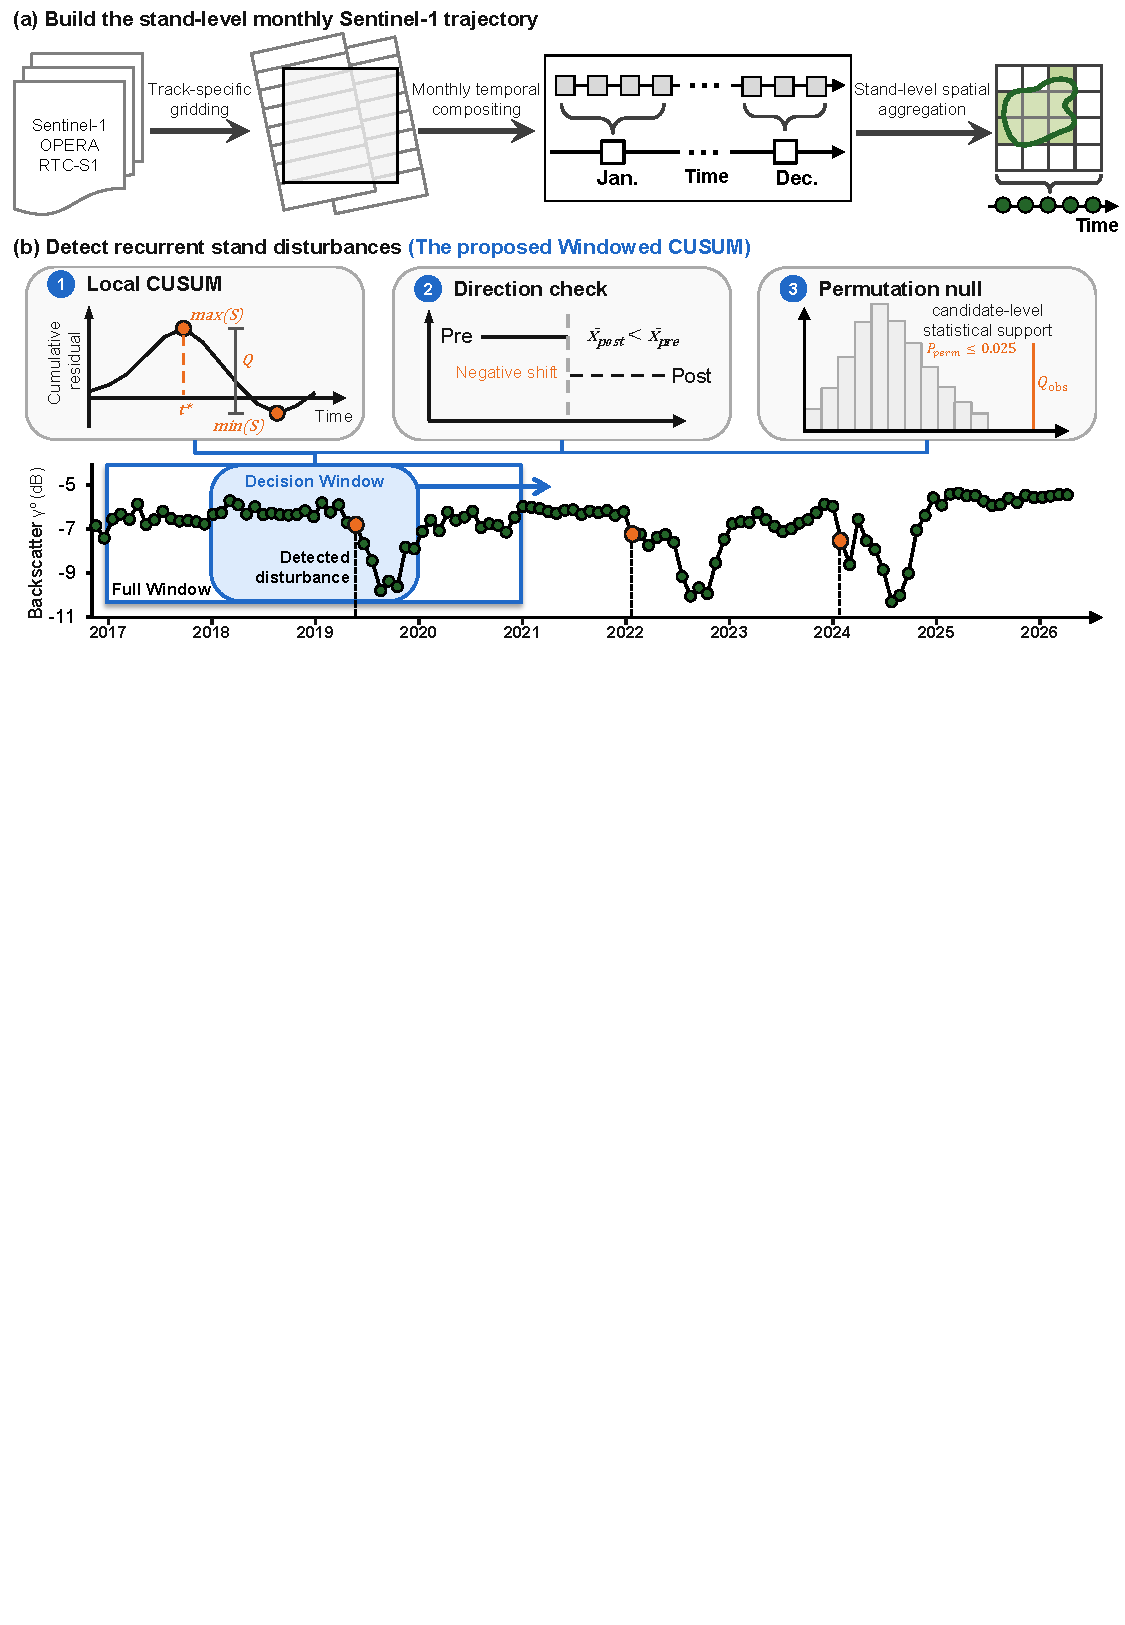
\includegraphics[width=0.85\linewidth]{figures/fig03_workflow.pdf}
    \caption{Overall methodological framework for recurrent stand-disturbance detection and plantation-rotation analysis.}
    \label{fig:workflow}
\end{figure}

\subsection{Sentinel-1 monthly time-series construction and stand representation}
\label{sec:s1_timeseries_representation}
Track-specific monthly series were constructed with S1-GRiTS (\url{https://github.com/ottoKae/S1-GRiTS}), retaining pass direction, relative orbit, and polarization. Let $\gamma_{\mathrm{dB},p,a,r}^{0,(q)}$ denote RTC backscatter for grid cell $p$, acquisition $a$, track $r$, and polarization $q\in\{\mathrm{VV},\mathrm{VH}\}$. Monthly backscatter was as shown in Equation~\eqref{eq:pixel_monthly_median}.
\begin{equation}
    \label{eq:pixel_monthly_median}
    y_{p,t,r}^{(q)}
    =
    \operatorname{median}
    \left\{
    \gamma_{\mathrm{dB},p,a,r}^{0,(q)}:
    a\in\mathcal{A}_{p,t,r}
    \right\},
\end{equation}
where $\mathcal{A}_{p,t,r}$ contains valid acquisitions in month $t$.
Missing months remained missing and were not interpolated.

For polygon $G_m$, the primary Polygon-first trajectory was the median of finite monthly values whose grid-cell centres fell within the polygon in Equation~\eqref{eq:polygon_monthly_median}. Grid cells contributed equally, and track-specific trajectories remained.
separate until event consolidation.
\begin{equation}
    \label{eq:polygon_monthly_median}
    x_{m,t,r}^{(q)}
    =
    \operatorname{median}
    \left\{
    y_{p,t,r}^{(q)}:
    \mathbf{c}_p\in G_m
    \right\}.
\end{equation}




Alternative spatial representations were evaluated to test the sensitivity of disturbance detection to stand representation. Polygon-first alternatives comprised the spatial mean, histogram mode, and nearest representative grid cell. Pixel-first alternatives retained individual grid-cell trajectories through disturbance detection and subsequently consolidated candidate evidence using eight-neighbour support, temporal DBSCAN, or joint space--time DBSCAN~\citep{Ester1996DBSCAN}. Parameters required by the Pixel-first strategies were selected exclusively from spatial training data as described in Section~\ref{sec:experimental_evaluation}.


\subsection{The proposed Windowed CUSUM}\label{sec:windowed_cusum}

The proposed Windowed CUSUM was designed to detect recurrent negative departures in stand-level Sentinel-1 backscatter using a sequence of overlapping local-reference windows. Each window establishes an updated local statistical context, allowing recurrent changes to be evaluated throughout the observation period without permanently segmenting the time series after each detected event. Figure~\ref{fig:windowed_cusum_concept} provides a visual overview of how overlapping local-reference windows, central-interval admission, the negative-shift constraint, and permutation screening jointly define an accepted candidate.

\begin{figure*}[pos=!htbp]
    \centering
    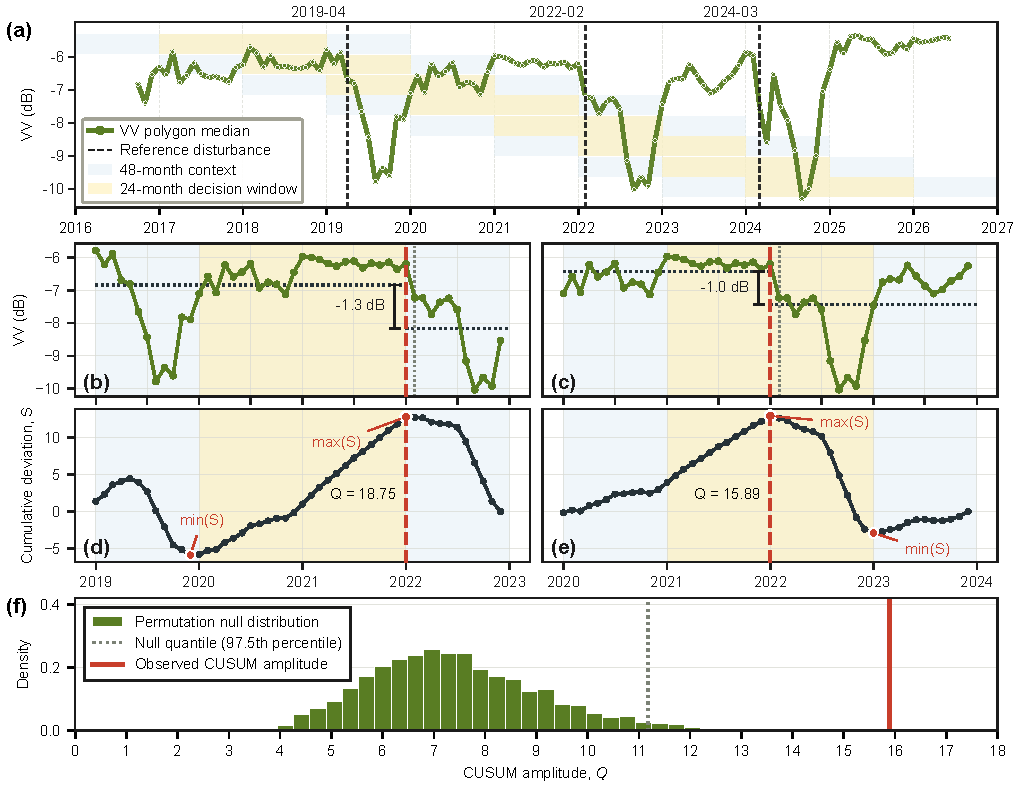
\includegraphics[width=\textwidth]{figures/fig04_windowed_cusum_concept.pdf}
    \caption{Conceptual illustration of Windowed CUSUM for one observed BALSA stand. (a) The stand-level VV trajectory with overlapping 48-month context windows, 24-month central decision windows, and dated disturbances. (b,c) Local-reference VV trajectories in two adjacent windows. (d,e) The corresponding cumulative-deviation curves: the candidate is rejected in (d) because it falls outside the central decision window, but retained in (e) because it falls within that window. (f) Evaluation of the retained CUSUM amplitude against its window-specific permutation null.}
    \label{fig:windowed_cusum_concept}
\end{figure*}


Windowed CUSUM was parameterized by the window length $W$ and the displacement $S$ between consecutive windows. For a window beginning at calendar month $b$, the full estimation window and central decision interval were defined as Equation~\eqref{eq:window_definition}. Each window required at least 12 finite observations; missing months were not interpolated, and boundary windows were clipped to the available record without temporal padding.
\begin{equation}
    \label{eq:window_definition}
    \mathcal{W}_b=[b,b+W),
    \qquad
    \mathcal{D}_b=[b+S,b+W-S),
\end{equation}
where $\mathcal{W}_b$ defines the temporal domain used to estimate the local CUSUM statistic, whereas $\mathcal{D}_b\subset\mathcal{W}_b$ defines the interval within which a candidate event can be admitted. The resulting decision-interval length is therefore $C=W-2S$. Thus, $W$ controls the local temporal context, while $S$ determines both the displacement between consecutive windows and the temporal margin excluded from candidate admission at each window boundary.


Within each local window, CUSUM was computed from the finite observations in temporal order. For notational simplicity, let $x_1,\ldots,x_n$ denote the finite observations extracted from the corresponding stand-level monthly trajectory, and let $\bar{x}$ denote their mean. The centred cumulative residual and CUSUM amplitude were defined in Equation~\eqref{eq:local_cusum}.
\begin{equation}
    S_t
    =
    \sum_{i=1}^{t}(x_i-\bar{x}),
    \qquad
    Q
    =
    \max_t S_t-\min_t S_t,
    \qquad
    t=1,\ldots,n .
    \label{eq:local_cusum}
\end{equation}
where $S_t$ is the cumulative residual at the $t$-th finite observation, $Q$ quantifies the magnitude of the strongest structural departure within the window, and $n$ is the number of finite observations. Thus, $S_t$ records the accumulated departure from the window mean as the trajectory is traversed chronologically, whereas $Q$ summarizes the overall strength of the resulting CUSUM signal.

For a persistent negative shift, positive deviations accumulate before the decline and negative deviations accumulate afterward. The cumulative residual therefore reaches a local maximum near the transition between the two states. The corresponding candidate change boundary was defined as~\citep{Page1954CUSUM,Ygorra2021CuSum} in Equation~\eqref{eq:candidate_position}.
\begin{equation}
    t^{*}
    =
    \arg\max_t S_t .
    \label{eq:candidate_position}
\end{equation}
Accordingly, $Q$ describes the magnitude of the local structural change, whereas $t^{*}$ identifies the candidate change location within the sequence of finite observations.



After mapping $t^*$ to calendar time, candidates outside $\mathcal{D}_b$ were discarded. Treating $x_{t^*}$ as the first post-change observation, we calculate in Equation~\eqref{eq:time_pre_post_mean}. A candidate was retained only when $\bar{x}_{\mathrm{post}}<\bar{x}_{\mathrm{pre}}$.
\begin{equation}
    \label{eq:time_pre_post_mean}
    \bar{x}_{\mathrm{pre}}
    =\operatorname{mean}(x_1,\ldots,x_{t^*-1}),
    \qquad
    \bar{x}_{\mathrm{post}}
    =\operatorname{mean}(x_{t^*},\ldots,x_n).
\end{equation}



Candidate support was evaluated against a window-specific permutation null rather than a common threshold on $Q$. Finite observations were randomly reordered and $Q$ recomputed for each permutation. The finite-sample-corrected $p$ value was in Equation~\eqref{eq:permutation_pvalue}~\citep{PhipsonSmyth2010Permutation}.
\begin{equation}
    p_{\mathrm{perm}}
    =
    \frac{
    1+\sum_{j=1}^{B}
    \mathbf{1}\{Q_j^{\mathrm{perm}}\ge Q_{\mathrm{obs}}\}
    }{B+1}.
    \label{eq:permutation_pvalue}
\end{equation}

The initial test used $B=3{,}999$; candidates with $0.015\le p_{\mathrm{perm}}\le0.035$ were recomputed with $B=19{,}999$. Candidates were retained at $p_{\mathrm{perm}}\le0.025$. This $p$ value refers only to the specified within-window null and is not a posterior disturbance probability or global false-discovery control.

Accepted candidates within one month were consolidated across overlapping windows and tracks. The representative month maximized track support, with the earliest month retained under ties.





\subsection{Experimental design and accuracy assessment}
\label{sec:experimental_evaluation}

\subsubsection{Reference-event protocol and spatial inference}


Historical signal characterization was separated from detector evaluation,
while spatial blocks were used to prevent information leakage and define
the unit of statistical resampling.

Absolute Sentinel-1 backscatter distributions were summarized from all valid polygon-month observations of the 3,498 validated BALSA polygons. Event-aligned analyses used the independently dated historical disturbance catalogue. For each polygon--track event, the pre-event background was defined as the median response from relative months $-12$ to $-3$ and required at least six finite observations. The paired event/post-event response was summarized over months 0 to $+2$ and required at least two finite observations. For the event-aligned trajectories, monthly responses were expressed relative to the same pre-event background and aligned by reference-event month. Track-specific responses were then fused by their median within each dated polygon event so that each event contributed once. These temporal-support criteria retained 1,018 events for the paired and event-aligned signature analyses, whereas all 1,093 reference-dated events from 462 polygons remained eligible for detector evaluation. Uncertainty in the paired and event-aligned signature summaries was estimated from 5,000 bootstrap resamples of complete spatial blocks.


The 1,093 reference events were grouped into 57 spatial blocks. All polygons, tracks, grid cells, and events from a block remained together. For analyses requiring parameter selection, the blocks were assigned to five event-balanced outer folds; parameters were selected on four folds and applied once to the held-out fold. The five held-out prediction sets were concatenated to obtain spatial out-of-fold estimates. Fixed-configuration analyses used the same blocks for paired inference without additional selection.



Detected and reference events were matched one-to-one within the prespecified $\pm2$-month tolerance, first maximizing the number of matches and then minimizing total absolute temporal lag. Precision, recall, and F1 were calculated at event level, and temporal mean absolute error (MAE) among matched pairs. Unmatched detections were not treated as independently verified false disturbances because the reference catalogue was not exhaustive.


The dated polygon event was therefore the unit of detector assessment, whereas the complete spatial block was the unit of statistical resampling. Paired 95\% confidence intervals for method and configuration contrasts were estimated from 5,000 bootstrap resamples of the 57 spatial blocks, using identical resamples for the quantities being compared~\citep{Davison1997Bootstrap}.


\subsubsection{Configuration sensitivity and component attribution}
\label{sec:configuration_component}

All configuration and component analyses followed the reference-event matching and spatial-inference protocol defined above. Whenever a representation or configuration required data-driven parameter selection, selection was restricted to the corresponding spatial training folds; analyses of locked configurations did not reopen parameter selection.

Sensitivity to stand representation was evaluated with the detector fixed at a 48-month window, 12-month displacement, and finite-sample permutation threshold of $p_{\mathrm{perm}}\leq0.025$. The Polygon-first median was compared with Polygon-first mean, histogram mode, and a representative-cell medoid, as well as Pixel-first connected support, temporal DBSCAN, and joint space--time DBSCAN~\citep{Ester1996DBSCAN}. Parameters required by the Pixel-first strategies were selected exclusively within the spatial training folds. Paired F1 contrasts were calculated relative to the Polygon-first median using the common spatial-block resampling protocol.

Window sensitivity evaluated $W\in\{24,36,48,60,72\}$ months and $S\in\{6,12\}$ months; 24/12 was excluded because its central decision interval was empty. A nested analysis selected geometry on the four training folds and evaluated it on the held-out fold. The previously locked 48/12 configuration remained unchanged for fixed operational analyses. Polarization sensitivity was evaluated under the retained Polygon-first representation and 48/12 geometry using VV-only, VH-only, either-polarization, and VV--VH agreement strategies.


Component attribution was evaluated only under the fixed operational configuration. The progressive analysis began with a single-pass Global CUSUM applied to the complete trajectory~\citep{Page1954CUSUM} and sequentially added local-reference windows, central-interval admission, the negative-shift constraint, and permutation-based screening. Only the complete configuration was designated the proposed Windowed CUSUM. A complementary controlled-removal analysis started from the complete detector and removed one component at a time while holding stand representation, missing-data treatment, candidate consolidation, track fusion, and event matching fixed. Adjacent progressive contrasts and full-minus-removed contrasts were evaluated using paired spatial-block resampling, with Holm adjustment applied to the four prespecified adjacent progressive comparisons. Reference polygons were additionally stratified by reference-event count to assess whether the effect of local-reference windowing was concentrated in recurrent-disturbance settings.


\subsubsection{Benchmark comparison and statistical robustness}
\label{sec:benchmark_robustness}

External benchmarking used the same reference catalogue, Polygon-first monthly trajectories, calendar support, event-matching rule, and spatial outer-fold structure defined above. Method-specific parameters were selected exclusively within the four spatial training folds before prediction on the held-out fold, and the five held-out prediction sets were concatenated for the final spatial out-of-fold comparison. Benchmark methods comprised maximum monthly decline, classical lower CUSUM~\citep{Page1954CUSUM}, ReCuSum~\citep{Ygorra2023ReCuSum}, a notebook implementation of factorized-polarization Bayesian online change-point detection~\citep{Bottani2026f-pol_BOCD}, and a BFAST-style seasonal one-break detector~\citep{Verbesselt2010BFAST}. Where decrease-filtered variants were evaluated, candidate events were additionally required to satisfy the same negative pre--post change direction used by Windowed CUSUM. Pairwise performance contrasts were quantified using the same paired spatial-block resampling scheme.

Temporal-null sensitivity changed only the permutation null while keeping the locked detector fixed. The finite-sample independent-value permutation~\citep{PhipsonSmyth2010Permutation} was compared with the previous empirical-rank implementation, 3-, 6-, and 12-month calendar-block permutations, residual moving-block-bootstrap nulls~\citep{Kunsch1989BlockBootstrap}, and a 3-month track-wise maximum-statistic null. All used an equivalent admission threshold of $p_{\mathrm{perm}}\le0.025$ and paired block inference. Monte Carlo stability was assessed across ten seeds for the stochastic null procedures. This analysis assessed robustness to temporal-null assumptions and did not reopen detector selection.








\subsubsection{Temporal truncation and prospective replay}
\label{sec:temporal_prospective}

Temporal truncation evaluated detection latency without changing the locked detector or the reference-event protocol defined above. For each historical reference event, the available Sentinel-1 record was truncated at $0$, $1$, $2$, $3$, $6$, and $12$ months after the reference month, and the fixed Windowed CUSUM configuration was replayed using only observations available up to the corresponding cutoff. No later observations were available to window construction, permutation screening, candidate consolidation, or track fusion. Recall and event-date stability were evaluated on a common-support cohort with sufficient temporal coverage at every horizon, allowing paired comparison without changes in the reference denominator. Uncertainty across truncation horizons was quantified using the same complete spatial blocks as the resampling units.

A separate prospective replay used observations available through June 2026 after all detector choices had been frozen. The 2026 manual review was excluded from representation, window, threshold, component, and benchmark selection. Candidate precision was estimated from a prespecified sample of detector-generated candidates, with the sampling fractions incorporated into the weighted estimates and spatial-block resampling used for uncertainty. Because review was conditioned on detected candidates rather than an independent sample of all disturbed and undisturbed polygons, the prospective analysis assessed candidate precision and operational behaviour but could not estimate missed disturbances or population recall.


\subsection{Stand-disturbance history reconstruction}
\label{sec:rotation_reconstruction}

The locked VV-only Windowed CUSUM was applied to each validated BALSA polygon to reconstruct its disturbance history during 2017--2025. For polygon $m$, the detected disturbance months were ordered as Equation~\eqref{eq:event_history} to form a temporally ordered event sequence,
\begin{equation}
    H_m^{(\mathrm{VV})}
    =
    (h_{m,1},h_{m,2},\ldots,h_{m,n_m}),
    \qquad
    h_{m,1}<h_{m,2}<\cdots<h_{m,n_m},
    \label{eq:event_history}
\end{equation}
where $h_{m,k}$ is the month of the $k$th detected disturbance and
$n_m$ is the observed stand-disturbance count. For spatial summaries,
$n_m$ was grouped as 0, 1, 2, and $\geq3$ detected disturbances.
The count refers only to disturbances observed within the Sentinel-1
record and therefore does not represent the absolute number of
plantation rotations.

Observed inter-disturbance intervals were calculated only between
consecutive detected disturbances in Equation~\eqref{eq:rotation_interval}.
\begin{equation}
    R_{m,k}^{\mathrm{obs}}
    =
    h_{m,k+1}-h_{m,k},
    \qquad
    k=1,\ldots,n_m-1,
    \label{eq:rotation_interval}
\end{equation}
where $R_{m,k}^{\mathrm{obs}}$ is the interval in months between adjacent
disturbance events. The first measurable interval therefore begins at
the first observed disturbance rather than the unknown planting date,
and intermediate events were never skipped to connect non-adjacent
disturbances. Uncertainty in interval summaries was estimated by
complete spatial-block bootstrap resampling.

Polarization robustness was assessed using a VH-supported subset of the
VV-defined intervals. An interval was classified as cross-polarization
consistent only when both bounding VV events had one-to-one VH matches
within $\pm2$ months. The original VV sequence was left unchanged:
unmatched intermediate VV events were retained and VH-only events were
not inserted. This subset was used only to assess polarization
sensitivity of the inter-disturbance interval distribution, not to
derive a separate VH-based rotation estimate.








% !TeX root = ../main.tex
\section{Results}\label{sec:results}

\subsection{Sentinel-1 signatures of historical stand disturbances}


Historical BALSA stand disturbances exhibited repeatable negative Sentinel-1 responses (Fig.~\ref{fig:s1_population_signatures}). The distributional analysis used all valid polygon-month observations from the 3,498 validated polygons; 1,018 events in 462 polygons had the paired temporal support required for the event-level summaries. Across all valid polygon-month medians, the 5th--95th percentile ranges were $-9.3$ to $-5.0$~dB for VV and $-15.7$ to $-11.5$~dB for VH. Median VV changed from $-6.0$~dB before disturbance to $-7.5$~dB during months 0 to $+2$, while VH changed from $-12.5$ to $-14.0$~dB. The pre- and post-event distributions nevertheless remained broadly overlapping, so neither polarization defined a stable national absolute threshold (Fig.~\ref{fig:s1_population_signatures}a).

\begin{figure}[pos=!htbp]
    \centering
    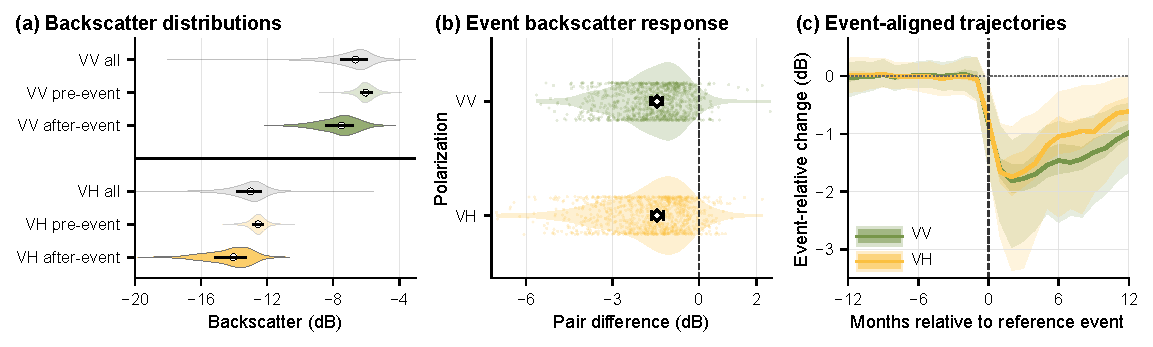
\includegraphics[width=1.0\textwidth]{figures/fig05_population_s1_signatures.pdf}
    \caption{Sentinel-1 signatures of historical balsa stand disturbances. (a) VV and VH distributions across all valid observations from the 3,498 validated BALSA polygons and during the pre-event ($-12$ to $-3$ months) and post-event (0 to $+2$ months) periods. (b) Paired post-minus-pre-event differences for 1,018 dated events; diamonds show medians and bars show 95\% complete-spatial-block bootstrap intervals. (c) Event-aligned changes relative to the pre-event background. Dark and light ribbons show interquartile ranges and pointwise 95\% block-bootstrap intervals, respectively.}
    \label{fig:s1_population_signatures}
\end{figure}
\FloatBarrier

Within-event contrasts were more consistent than the absolute values. Median post-minus-pre-event backscatter was $-1.5$~dB for VV (95\% complete-spatial-block bootstrap interval, $-1.7$ to $-1.3$~dB) and $-1.5$~dB for VH ($-1.6$ to $-1.2$~dB); 96.4\% and 94.1\% of the respective changes were negative (Fig.~\ref{fig:s1_population_signatures}b). The median deviations reached approximately $-1.8$~dB by month $+2$ and remained negative at month $+12$ ($-1.0$~dB for VV and $-0.6$~dB for VH). Pointwise 95\% spatial-block bootstrap intervals remained below zero from month 0 through month $+12$ for both polarizations (Fig.~\ref{fig:s1_population_signatures}c).


The representative polygon showed the same stand-scale response
(Fig.~\ref{fig:timeseries_signature}). Polygon-level median and mean
trajectories preserved the major disturbance valleys, and the March 2024
reference event coincided with coherent VV/VH declines and an optical
transition from dense canopy to exposed ground. Similar absolute
backscatter levels occurred during recovery and subsequent disturbance,
further supporting characterization relative to each stand's recent state.


\begin{figure}[pos=!htbp]
    \centering
    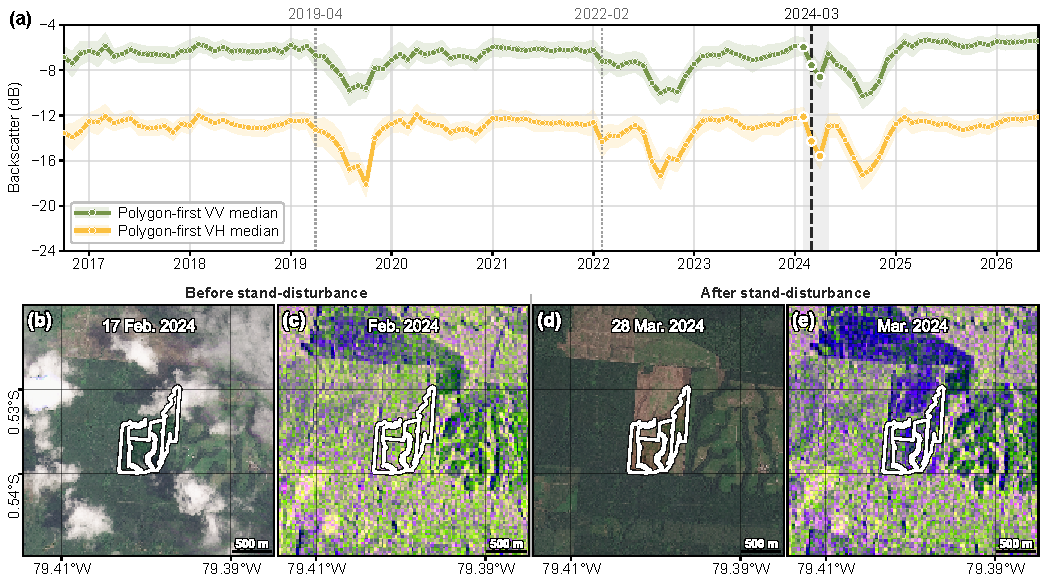
\includegraphics[width=\linewidth]{figures/fig06_representative_timeseries.pdf}
    \caption{Sentinel-1 and optical observations of a representative balsa plantation. (a) Monthly Polygon-first VV and VH median backscatter from October 2016 to June 2026. Shading denotes the within-polygon pixel interquartile range for each polarization, and vertical lines mark independently interpreted reference-event months. (b,c) PlanetScope and Sentinel-1 observations before the March 2024 event. (d,e) Corresponding observations after the event. Sentinel-1 false-colour composites use R = VV, G = VH, and B = VV$-$VH; scale bars represent 500~m.}
    \label{fig:timeseries_signature}
\end{figure}
\FloatBarrier



\subsection{Stand representation and configuration sensitivity}
\label{sec:representation_configuration}




We next evaluated the sensitivity of disturbance detection to stand representation, temporal window geometry, and polarization strategy.


\begin{figure*}[pos=!htbp]
    \centering
    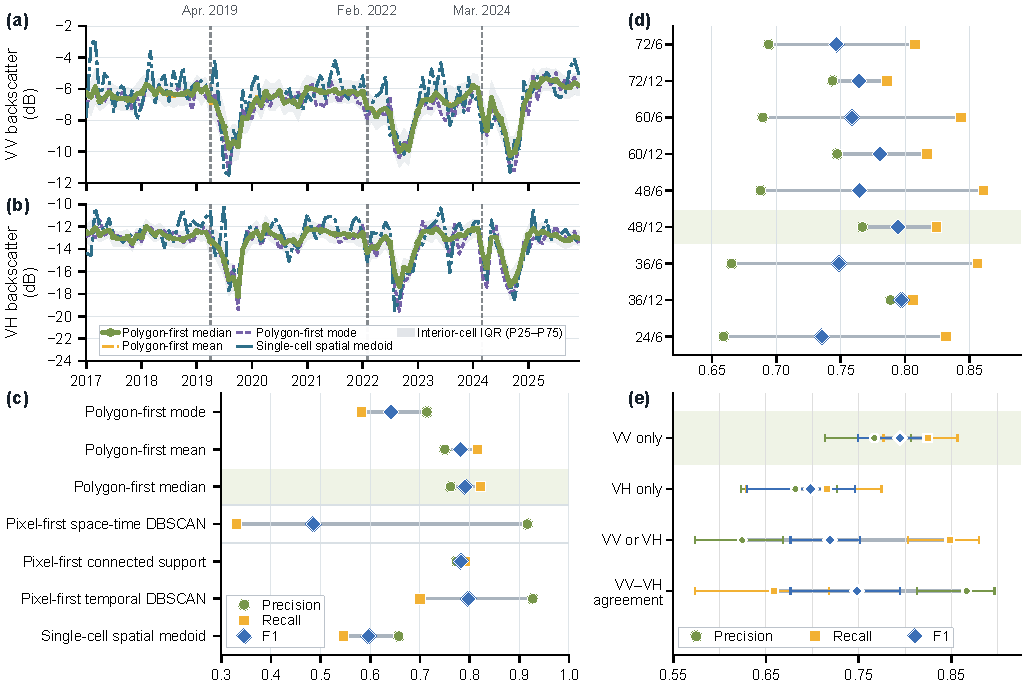
\includegraphics[width=\linewidth]{figures/fig07_representation_configuration.pdf}
    \caption{Sensitivity of Windowed CUSUM to stand representation, temporal window geometry, and polarization strategy. (a,b) Illustrative VV and VH stand trajectories with cell-level interquartile ranges and reference disturbances. (c--e) Event-level precision, recall, and F1 across stand representations, window configurations, and polarization strategies, respectively. Whiskers denote 95\% spatial-block bootstrap confidence intervals, and pale-green highlighting indicates the retained configurations.}
    \label{fig:stand_representation_sensitivity}
\end{figure*}

Under the fixed 48/12 configuration, the Polygon-first median achieved precision 0.762, recall 0.823, and F1 0.791 (Fig.~\ref{fig:stand_representation_sensitivity}~(c)). Alternative representations produced no detectable F1 improvement; even temporal DBSCAN, which had the highest alternative point estimate (F1 = 0.798), differed from the median by only $+0.007$ (95\% CI: $-0.032$ to 0.042). The Polygon-first median was therefore retained because it preserved high recall without requiring pixel-support or clustering parameters.


Across the evaluated window geometries, 12-month displacements generally favored F1 over six-month displacements (Fig.~\ref{fig:stand_representation_sensitivity}~(d)). The highest fixed F1 was 0.797 for 36/12, only 0.003 above the prospectively locked 48/12 configuration (95\% CI: $-0.013$ to 0.019). Although 36/12 was selected in all five outer folds, nested spatial out-of-fold F1 was 0.796. The prespecified 48/12 geometry was therefore retained.



VV-only detection produced the highest F1 (0.795; precision 0.767, recall 0.824; Fig.~\ref{fig:stand_representation_sensitivity}~(e)). Either-polarization fusion increased recall but reduced precision, whereas VV--VH agreement produced the opposite trade-off; neither improved F1. VV was therefore retained as the operational input.



\subsection{Component attribution of the proposed Windowed CUSUM}
\label{sec:representation_component_ablation}


Progressive component analysis identified local-reference windowing and central-interval admission as the two largest incremental contributors (Table~\ref{tab:component_ablation}). Windowing primarily increased recall ($\Delta F1=+0.137$, 95\% CI: 0.075--0.198), whereas the central interval recovered precision ($\Delta F1=+0.127$, 0.103--0.146). Permutation screening provided a further F1 gain of 0.036 (0.022--0.049), while the negative-shift constraint had negligible discriminative effect.


\begin{table*}[pos=!htbp]
    \centering
    \small
    \caption{Progressive component analysis under the fixed 48/12 configuration. $\Delta F1$ compares adjacent configurations; intervals are paired spatial-block bootstrap 95\% CIs.}
    \label{tab:component_ablation}
    \begin{tabular}{lccccc}
        \toprule
        Cumulative configuration
        & Detections
        & Precision
        & Recall
        & F1
        & Incremental $\Delta F1$ [95\% CI] \\
        \midrule

        Global CUSUM
        & 447
        & 0.852
        & 0.349
        & 0.495
        & -- \\

        + Local-reference windows
        & 1,948
        & 0.493
        & 0.878
        & 0.631
        & $+0.137$ [0.075, 0.198] \\

        + Central decision interval
        & 1,362
        & 0.684
        & 0.852
        & 0.758
        & $+0.127$ [0.103, 0.146] \\

        + Negative-shift constraint
        & 1,350
        & 0.687
        & 0.848
        & 0.759
        & $+0.000$ [$-0.003$, 0.003] \\

        + Permutation-based screening
        & 1,175
        & 0.767
        & 0.824
        & \textbf{0.795}
        & $+0.036$ [0.022, 0.049] \\

        \bottomrule
    \end{tabular}
\end{table*}


Additional controlled removal produced the same ordering. The full-minus-removedF1 contrast was largest for local-reference windowing ($+0.327$, 95\% CI: 0.280--0.370), compared with $+0.038$ for the central interval and $+0.036$ for permutation screening; removal of the negative-shift constraint had negligible effect. Both analyses therefore identified local-reference windowing as the principal source of recurrent-event sensitivity.


\FloatBarrier


\subsection{Benchmark comparison and statistical robustness}
\label{sec:benchmark_null_sensitivity}

For external benchmarking, Windowed CUSUM achieved precision 0.787, recall 0.805, F1 0.796, and temporal MAE 0.778 months (Table~\ref{tab:benchmark_comparison}). The strongest alternative, decrease-filtered ReCuSum, matched its precision (0.787) but had lower recall (0.591; F1 = 0.675), yielding a paired F1 advantage of $+0.122$ (95\% CI: 0.094--0.149). The benchmark advantage therefore arose primarily from recurrent-event recall.


\begin{table}[pos=!htbp]
    \centering
    \small
    \caption{Nested five-fold spatial out-of-fold comparison of disturbance detectors using common Polygon-first median trajectories and a $\pm2$-month event-matching tolerance. Temporal MAE was calculated for matched events only.}
    \label{tab:benchmark_comparison}

    \begin{tabular}{lcccc}
        \toprule
        Method
        & Precision
        & Recall
        & F1
        & MAE (months) \\
        \midrule

        \textbf{Windowed CUSUM}
        & 0.787
        & 0.805
        & \textbf{0.796}
        & 0.778 \\

        ReCuSum, decrease-filtered
        & 0.787
        & 0.591
        & 0.675
        & 0.752 \\

        f-pol BOCD, decrease-filtered
        & 0.740
        & 0.343
        & 0.469
        & 0.747 \\

        ReCuSum, raw
        & 0.419
        & 0.513
        & 0.461
        & 0.743 \\

        Maximum monthly decline
        & 0.335
        & 0.572
        & 0.422
        & 0.755 \\

        Classical lower CUSUM
        & 0.171
        & 0.290
        & 0.215
        & 1.498 \\

        BFAST-style, decrease-filtered
        & 0.679
        & 0.101
        & 0.175
        & 0.673 \\

        \bottomrule
    \end{tabular}
\end{table}



Separately, temporal-null formulation altered the precision--recall operating point (Table~\ref{tab:temporal_null_sensitivity}). Finite-sample correction of the independent-value permutation changed F1 only from 0.791 to 0.795. In contrast, preserving temporal dependence made screening more selective. A three-month calendar-block permutation increased precision from 0.767 to 0.828 but reduced recall from 0.824 to 0.676 ($\Delta F1=-0.050$, 95\% CI: $-0.084$ to $-0.028$), with stronger dependence-preserving formulations producing still lower recall. Monte Carlo seed variation was negligible relative to differences among null formulations. Under the common threshold, the finite-sample independent-value permutation retained the highest F1.


\begin{table*}[pos=!htbp]
    \centering
    \small
    \caption{Sensitivity of Windowed CUSUM to alternative temporal-null formulations for permutation-based screening under the fixed 48-month window, 12-month displacement, and $\pm2$-month event-matching tolerance. MBB denotes residual moving-block bootstrap and maxT denotes a track-wise maximum-statistic block null.}
    \label{tab:temporal_null_sensitivity}

    \begin{tabular}{llcccc}
        \toprule
        Temporal-null formulation
        & Block length
        & Detections
        & Precision
        & Recall
        & F1 \\
        \midrule

        Archived empirical-rank IID implementation
        & --
        & 1,180
        & 0.762
        & 0.823
        & 0.791 \\

        \textbf{Finite-sample-corrected IID permutation}
        & --
        & 1,175
        & 0.767
        & 0.824
        & \textbf{0.795} \\

        Calendar-block permutation
        & 3 months
        & 892
        & 0.828
        & 0.676
        & 0.745 \\

        Calendar-block permutation
        & 6 months
        & 410
        & 0.902
        & 0.339
        & 0.492 \\

        Calendar-block permutation
        & 12 months
        & 0
        & --
        & 0.000
        & 0.000 \\

        Residual MBB
        & 3 months
        & 927
        & 0.790
        & 0.670
        & 0.725 \\

        Residual MBB
        & 6 months
        & 830
        & 0.772
        & 0.586
        & 0.667 \\

        Residual MBB
        & 12 months
        & 897
        & 0.761
        & 0.625
        & 0.686 \\

        Track-wise maxT block null
        & 3 months
        & 272
        & 0.915
        & 0.228
        & 0.365 \\

        \bottomrule
    \end{tabular}
\end{table*}

Dependence-aware temporal nulls produced a clearer precision--recall trade-off. A three-month calendar-block permutation increased precision from 0.767 to 0.828 but reduced recall from 0.824 to 0.676, lowering F1 to 0.745 ($\Delta F1=-0.050$, 95\% CI: $-0.084$ to $-0.028$). Increasing the block length made candidate admission progressively more conservative; recall declined to 0.339 with six-month blocks, while the 12-month formulation admitted no events. The track-wise maximum-statistic block null showed a similar pattern, achieving precision of 0.915 but recall of only 0.228 (F1 = 0.365).

Residual moving-block-bootstrap nulls produced intermediate results, with F1 ranging from 0.667 to 0.725 across block lengths of 3--12 months. Monte Carlo variation across random seeds was negligible relative to the differences among temporal-null formulations. Under the common $p_{\mathrm{perm}}\leq0.025$ threshold, the finite-sample-corrected IID permutation produced the highest overall F1, whereas increasingly dependence-preserving nulls systematically shifted the detector toward higher selectivity and lower recall.

\subsection{Temporal truncation and prospective performance}
Temporal truncation showed that detection sensitivity increased substantially as post-disturbance observations accumulated. Among the 1,065 reference events evaluable at every horizon, recall increased from 0.202 using observations available only through the reference month to 0.613 after three months, 0.790 after six months, and 0.849 after 12 months. Event dates were comparatively stable once detections had been established: of the 841 reference events detected by the six-month horizon, 814 (96.8\%) were assigned a disturbance month within two months of their corresponding 12-month estimate.

When the locked Windowed CUSUM configuration was subsequently replayed using observations through June 2026, it produced 139 provisional disturbance candidates. Manual review was conducted for 95 sampled candidate polygons. After accounting for the tier-specific sampling fractions, 57.5\% of candidates were estimated to represent confirmed disturbances (95\% spatial-block bootstrap CI: 0.287--0.812), increasing to 64.0\% (95\% CI: 0.393--0.846) when probable disturbances were also included.
\FloatBarrier

\subsection{Recurrent disturbance intervals and plantation rotation dynamics}
\label{sec:rotation_dynamics}

Applying the VV-only Windowed CUSUM to all validated BALSA polygons identified 6,658 qualified disturbance events during 2017--2025. Among these, 2,194 polygons contained at least two events and provided 3,509 intervals between consecutive disturbances. As shown in Fig.~\ref{fig:national_recurrence_patterns}~(d), the median observed inter-disturbance interval was 36 months (IQR: 22--46 months; 95\% spatial-block bootstrap CI: 35--38 months). More than half of all intervals (53.0\%) occurred between 24 and 47 months, and 74.3\% were at least 24 months. Short intervals were also present, with 20.4\% shorter than 12 months, indicating that not every pair of successive detections can be interpreted as a complete plantation rotation.

\begin{figure*}[pos=!htbp]
    \centering
    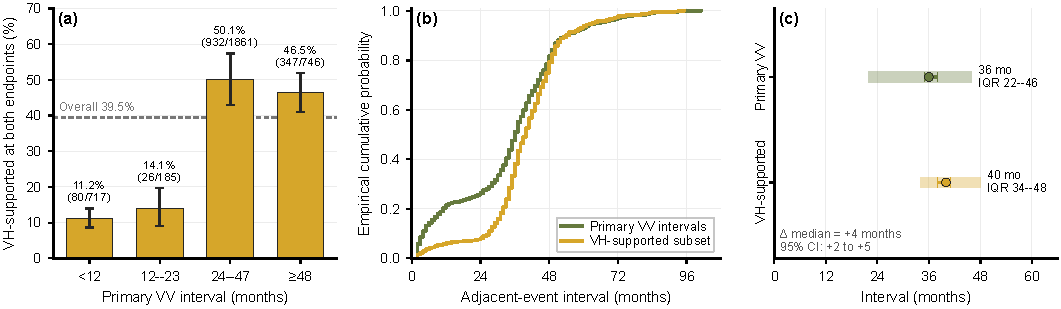
\includegraphics[width=\linewidth]{figures/fig08_polarization_intervals.pdf}
    \caption{Cross-polarization sensitivity of observed inter-disturbance intervals. (a) Fraction of VV-defined intervals for which both bounding disturbance events had corresponding VH detections within $\pm2$ months. (b) Empirical cumulative distributions of all VV intervals ($n=3{,}509$) and the cross-polarization-consistent subset ($n=1{,}385$). (c) Median and interquartile interval estimates with 95\% spatial-block bootstrap confidence intervals.}
    \label{fig:polarization_interval_sensitivity}
\end{figure*}

To assess whether the approximately three-year recurrence was specific to the VV-derived disturbance sequence, we performed a cross-polarization robustness analysis using VH. Cross-polarization filtering retained 1,385 intervals from 1,081 polygons (39.5\% of VV intervals). Their median was 40 months (IQR: 34--48; 95\% CI: 38--41), four months longer than the primary VV estimate (paired 95\% CI: $+2$ to $+5$ months), indicating that the dominant approximately three-year recurrence persisted with VH support. VH support was substantially less frequent for intervals shorter than
24 months than for longer intervals, indicating preferential retention of longer recurrence periods rather than an unbiased refinement of the VV estimate.



These intervals represent recurrent stand turnover observed within the Sentinel-1 record. Notably, individual negative disturbance events could not always be independently attributed to clear-cut harvesting. The 36-month median is therefore interpreted as a rotation-relevant recurrence timescale of observed plantation turnover.

Application of the VV-only Windowed CUSUM to 3,498 validated BALSA polygons identified 6,658 disturbance events during 2017--2025 (Fig.~\ref{fig:national_recurrence_patterns}). Event recurrence showed marked spatial heterogeneity (Fig.~\ref{fig:national_recurrence_patterns}~(a)), while annual detections ranged from 308 in 2023 to 1,026 in 2022 (Fig.~\ref{fig:national_recurrence_patterns}~(b)). The 2023 minimum coincided with the post-boom contraction that followed the 2019--2021 balsa fever, when exceptional wind-sector demand rapidly depleted mature plantation stocks and Ecuadorian balsa exports subsequently declined sharply~\citep{Sanchez2023BalsaExports,EIA2024IllWind}. As shown in Fig.~\ref{fig:national_recurrence_patterns}~(c), 82.9\% of the inventory contained one to three detected events and 349 plots contained none. The 2,194 stands with at least two events provided 3,509 consecutive inter-disturbance intervals, with a median of 36 months (IQR: 22--46 months; 95\% spatial-block bootstrap CI: 35--38 months; Fig.~\ref{fig:national_recurrence_patterns}d).

\FloatBarrier

% !TeX root = ../main.tex
\section{Discussion}\label{sec:discussion}


\subsection{Local reference solves recurrent-event sensitivity}
Recurrent balsa disturbances were expressed more consistently as temporal departures from each stand's recent state than as fixed backscatter levels. Absolute VV and VH distributions overlapped substantially, whereas reference-dated disturbances showed repeatable negative within-stand responses. This supports a local-reference formulation. After one disturbance and subsequent recovery, a renewed decline can be evaluated relative to the updated stand state rather than against a fixed national threshold. Previous Sentinel-1 CUSUM approaches have demonstrated the value of cumulative temporal departures for tropical forest-disturbance monitoring~\citep{Ygorra2021CuSum,Aquino2022RadarDisturbance}, while ReCuSum extended this principle through recursive segmentation~\citep{Ygorra2023ReCuSum}. Windowed CUSUM instead repeatedly establishes overlapping local contexts without permanently partitioning the trajectory.

The component analyses showed that local-reference windowing was the main source of recurrent-event sensitivity, whereas central-interval admission and permutation screening primarily recovered precision. This mechanism is also consistent with the benchmark comparison, in which the proposed method's advantage arose mainly from higher event recall. Polygon-first median aggregation provided a complementary benefit. It represented the plantation management unit directly and required few additional parameters. The connected-support Pixel-first route slightly increased precision but reduced recall, and its paired F1 difference from Polygon-first included zero. Detection nevertheless required post-disturbance temporal context, indicating that the method is better suited to recurrent-event reconstruction and delayed monitoring than to immediate change alerting.






\subsection{Observed balsa turnover has a dominant 3-year timescale}

The median 36-month interval between consecutive detected disturbances represents the principal plantation-level finding. This interval should be interpreted as an observed recurrence timescale rather than a direct planting-to-harvest age, but it is consistent with the rapid growth and commercial management of balsa in Ecuador. Producer surveys in Los R\'ios report harvesting or purchasing commonly around three to four years~\citep{GonzalezOsorio2010Balsa}, while Ecuadorian growth studies show rapid early development and strong site-dependent productivity~\citep{CanadasLopez2019BalsaGrowth}. Age-related wood-property measurements from approximately 30--40-month-old stands provide additional biological context~\citep{Moya2025BalsaProperties}. The observed 36-month central tendency therefore falls within a plausible commercial development period.

Cross-polarization analysis supported the persistence of this approximately three-year pattern, although requiring VH evidence at both bounding events shifted the median from 36 to 40 months. Because VH agreement preferentially retained longer intervals, the latter should not be interpreted as a corrected rotation estimate. Rotation length is also unlikely to be universal: balsa systems in Papua New Guinea commonly operate on longer, approximately five- to six-year cycles~\citep{Jenkin2019BalsaValueChain,Midgley2010Balsa}. Site productivity, management, and market conditions can therefore alter the relationship between disturbance recurrence and biological rotation.

The distinction is important because planting dates were unavailable, the first and last cycles were censored by the observation period, and not every negative disturbance could be independently attributed to clear-cut harvesting. Very short intervals may instead reflect partial clearing, multi-stage disturbance, or unresolved event structure. The 36-month estimate is therefore best interpreted as a rotation-relevant timescale of recurrent stand turnover within the monitored inventory rather than a direct estimate of biological rotation age.





\subsection{Robustness, limitations, and transferability}

Spatially blocked evaluation reduced the optimistic bias that can arise when geographically related observations are divided between parameter selection and evaluation~\citep{Roberts2017SpatialCV}, but it does not replace external geographic validation. Performance may differ under other rainfall regimes, terrain, acquisition geometries, stand structures, or management systems. The temporal-null analysis further showed that permutation screening depends on how temporal dependence is represented: dependence-preserving nulls increased selectivity but substantially reduced recall. The retained independent-value permutation should therefore be viewed as an operational precision--recall choice under the evaluated threshold rather than evidence that monthly Sentinel-1 observations are temporally exchangeable.

Disturbance attribution remains another limitation. Negative Sentinel-1 transitions can be associated with harvesting but may also reflect partial canopy removal, flooding, wind damage, or observation effects, and forest-disturbance accuracy depends strongly on reference design and disturbance definition~\citep{RodriguezPaulino2024Review}. The candidate-conditioned 2026 review therefore informs prospective candidate precision but cannot estimate missed disturbances or population recall. Accordingly, detected-event counts should not be interpreted directly as verified harvested area.

The transferable contribution is the combination of track-specific SAR time series, stand-level representation, recurrent local-reference detection, and spatially structured evaluation while maintaining a clear distinction between observed disturbance recurrence and biological rotation. Future work should focus on reducing detection latency and developing dependence-aware statistical screening that preserves realistic temporal structure without the large recall losses observed here.




% !TeX root = ../main.tex
\section{Conclusion}
\label{sec:conclusion}

This study establishes Windowed CUSUM as a local-reference framework for reconstructing recurrent stand disturbances from near-decadal Sentinel-1 SAR time series. This is the first study to use a near-decadal Sentinel-1 record to reconstruct multiple stand-level disturbance events and derive rotation-relevant temporal dynamics in a short-rotation plantation system. Rather than relying on a single historical baseline or recursively partitioning the time series after each detected change, Windowed CUSUM repeatedly evaluates overlapping local temporal contexts and separates the statistical estimation domain from the central interval in which events are admitted. This design accommodates evolving harvest--regrowth trajectories while retaining month-level event timing. Under nested five-fold spatial out-of-fold evaluation, the method achieved a precision of 0.789, recall of 0.806, and F1 of 0.797, outperforming the strongest benchmark primarily through improved recall. Component analyses further identified local-reference windowing as the principal source of this gain.



The methodological advance is therefore not limited to improved disturbance-detection accuracy. Windowed CUSUM converts a continuous, cloud-independent SAR record into temporally explicit histories of repeated stand turnover, extending Sentinel-1 monitoring from individual forest-loss events toward reconstruction of multi-cycle plantation dynamics. Across the validated BALSA inventory, these histories yielded a median interval of 36 months between consecutive disturbances, consistent with the rapid growth and short management cycles reported for balsa in Ecuador and providing an independent plausibility check on the reconstructed rotation. More broadly, the framework demonstrates the value of dense SAR archives for reconstructing short-rotation plantation dynamics in cloud-prone regions where optical observations lack sufficient temporal continuity.






% !TeX root = ../main.tex
\section*{Data and code availability}

% TODO(release): Replace OWNER and add the archival DOI before submission.
The maintained Windowed CUSUM source, frozen configuration, experiment drivers, compact result tables, and provenance manifests will be available at \url{https://github.com/OWNER/windowed_CUSUM_balsa}. Large S1-GRiTS Zarr cubes and derived pixel caches are not included in Git because of their size. The radar source is the publicly available NASA OPERA RTC-S1 archive; access conditions for official Ecuadorian plantation boundaries and historical management records follow those of their data providers. A versioned archival DOI will be added to the published data and code statement if one is issued before submission.

\section*{Ethics declaration}

The study used satellite observations, administrative plantation polygons, and historical stand-event records. It did not involve human participants, personal data, or animal experiments.

\section*{Conflict of interest}

The authors declare that they have no known competing financial interests or personal relationships that could have influenced the work reported in this article.

\section*{Funding}

This work was supported by the Startup Research Fund of Henan Academy of Sciences (No.~242025005) and the Open Research Fund Program of the MNR Key Laboratory for Geo-Environmental Monitoring of the Great Bay Area.

\section*{Declaration of generative AI and AI-assisted technologies}

During manuscript revision, the authors used OpenAI Codex to assist with repository auditing, reproducible workflow execution, code organization, and English-language editing. The authors reviewed the generated material, verified numerical results against the experiment outputs, revised the content where necessary, and take full responsibility for the published article.


\printcredits
\bibliographystyle{cas-model2-names}
\bibliography{references}

\end{document}
